% !TeX spellcheck = de_DE_frami
\documentclass[12pt]{article}
%\documentclass[12pt,a4paper,titlepage]{scrartcl}
%\usepackage[left=2cm,right=2.5cm,top=2.5cm,bottom=2cm]{geometry}
\usepackage[onehalfspacing]{setspace}
\usepackage[ngerman]{babel}
\usepackage[hidelinks]{hyperref}
\usepackage{verbatim} % for multiline comments
\usepackage{graphicx}
\graphicspath{ {./images/} }

% text-library
\usepackage[backend=biber, style=numeric]{biblatex}
\DefineBibliographyStrings{ngerman}{
	bibliography = {References},
}
\addbibresource{sources.bib}

\usepackage{graphicx}
\graphicspath{ {./images/} }

\begin{document}

\begin{titlepage}	
	\title{\LARGE Seminararbeit\\ \large Algorithmisches Handeln mit Cryptowährungen}
	\date{\small \today}
	\author{\small Carl Heinrich Bellgardt}	
	\clearpage\maketitle
	\thispagestyle{empty}
\end{titlepage}

\setcounter{page}{2}
\tableofcontents
\pagebreak
\section{Einleitung}
\subsection{Handeln, minimalistisch und computergesteuert}
	Maschinen existieren nur zu einem Zweck: dem Menschen die Arbeit zu erleichtern. Das gilt auch für Computer. Sie sind Rechenmaschinen der Superlative, denn Sie rechnen in einem Tempo, bei dem kein Mensch mithalten kann. \glqq Die Prozessor-Leistung für Computer verdoppelt sich alle 2 Jahre\grqq{} (\cite{}),  so lautet die neue Version des Mooreschen Gesetztes. Es ist eigentlich zwar kein Gesetz, sondern eher eine Faustregel, hat sich allerdings über einen langen Zeitraum bewahrheitet. Es macht uns klar, in welchem rasanten Tempo Rechenleistungen steigen. So wundert es auch keinen, dass Computer bereits in allen Bereichen unseres Lebens Fuß gefasst haben, ob im Alltag, in der Industrie, oder auch bei Expeditionen in den Weltraum, die ohne solche Technik undenkbar wären. Sie werden gebraucht, wenn kein Mensch in der Lage ist, eine Rakete so präzise in Echtzeit zu steuern, Schaltkreise in Platinen zu löten, die mit bloßem Auge nicht sichtbar sind, oder tausende Pakete am Tag zu sortieren und den Überblick in einfach allem zu behalten.\\
	Gibt es überhaupt etwas, was Computer nicht können?\\
	Bis heute sind Maschinen nicht in der Lage zu denken. Jedes Programm ist nur ein fester Ablauf, ein vordefinierter Algorithmus, welcher vom Computer souverän ausgeführt wird. Jede Maschine ist nur auf eine oder wenige verschiedene spezifische Aufgaben ausgerichtet. Zwar gibt es bereits Künstliche Intelligenzen\footnote{Im folgenden als \glqq KI\grqq{} bezeichnet}, welche mittels maschinellen Lernens vereinfacht unser Lernverhalten imitieren. Jedoch sind diese noch in der Anfangsphase und nur bei Gegebenheit vieler Voraussetzungen in sehr spezifischen Aufgaben einsetzbar. Letztlich handelt es sich auch dabei um reine Mathematik - Berechnungen, das einzige was ein Computer kann. Nichts desto trotz gibt es erste Erfolge, wie selbstfahrende Autos, allerdings sind diese noch nicht völlig ausgereift, stoßen oft an ihre Grenzen und funktionieren nur aufgrund der unvorstellbar großen Datenmenge an Übungsmaterialien, die zum Trainieren der KIs zur Verfügung stehen.\\
	Ich selber habe schon früh begonnen, Aufgaben an selbst geschriebene Programme oder Macros zu übergeben, um mir die Arbeit zu erleichtern. Manchmal habe ich nur automatisiert Dateien verschoben und manchmal hat mein Script an der Bildschirmfarbe erkannt, welche Taste es im Computerspiel drücken muss. Auch kleine Simulationen, wie zum Beispiel der Test von Roulettestrategien, lassen sich problemlos in wenigen Sekunden mehrere Millionen Male durchführen, denn Computer arbeiten schnell und effizient.\\
	\glqq Ein Risiko entsteht, wenn du nicht weißt, was du tust. \grqq{} (\cite{ChristophRottwilm}) Dieses Zitat stammt von Warren Buffet, einem der größten Investoren der Welt, und es bezieht sich auf den Aktienhandel, ein Themengebiet, das für seine Komplexität und Vielschichtigkeit bekannt ist. Das Zitat gilt auch heute noch, vermutlich mehr als jemals zuvor, aber für mich stellt sich die Frage: Wann weiß ich, was ich tue?\\
	Im Bereich des Aktienhandels gibt es bereits eine Vielzahl mathematischer Vorgehensweisen zur Berechnung von Faktoren und Strategien. Oft kommen diese Ergebnisse allerdings nur bei der Visualisierung zum Einsatz und werden eher als eine Art Handelsempfehlung gesehen und dann von einer Person mehr oder weniger ungenau und nach Gefühl interpretiert. Das Vertrauen in eine Maschine ist geringer als in einen Menschen, zu groß ist die Angst davor, einen Faktor zu übersehen, auf den der Computer nicht programmiert ist, den ein Mensch aber erkennen und spontan darauf reagieren kann.\\
	Ist es also denkbar, auf Bauchgefühl und Intuition, also auf Erfahrung und eigenes Denken zu verzichten und stattdessen nach einem festen Muster, also einem Algorithmus, zu handeln? Kann man sich auf Indikatoren, reine mathematische Formeln, verlassen, und den Mensch durch die immense Rechenkraft der Maschine ersetzen? Ziel dieser Arbeit ist es, herauszufinden, ob anhand von Indikatoren eine erfolgreiche Handelsstrategie umsetzbar ist. Wie schwer ist es, einen Handelsalgorithmus der simpelsten Art zu erstellen, der auch noch rentabel ist? Bereits existierende Indikatoren, also mathematisch berechenbare Anzeiger für beispielsweise Kursentwicklungen, sind ein einfacher Weg Vorhersagen zu treffen und eignen sich damit hervorragend für einen solchen Algorithmus. Und zuletzt, da wir mit Maschinen arbeiten, die ohne Probleme Milliarden von Berechnungen in der Sekunde durchzuführen in der Lage sind, wird das fertige Produkt auch auf seinen Profit mittels Backtesting \footnote{Engl. Back: Zurück. Simulation oder Test mit historischen Daten.} untersucht.

\subsection{Cryptowährungen}
	\subsubsection{Was sind Cryptowährungen?}
		Bitcoin wurde 2009 geschaffen, um eine Alternative zu den von Regierungen zentralisierten und kontrollierten Fiatwährungen zu bieten. Bitcoin war die erste Währung seiner Art, abgesichert durch das dezentrale Rechnernetz, mit einer transparenten Blockchain, um alle Transaktionen in kürzester Zeit durchführen zu können. Schnell sind Cryptowährungen aber auch durch ihre digitale Umsetzung und die daraus resultierende globale Verfügbarkeit von der Handelsbranche entdeckt worden. Durch die hohe Volatilität\footnote{auch Standardabweichung}, also die starken Preisschwankungen der meisten Cryptowährungen, lässt sich viel schneller, wenn auch risikoreicher, durch reinen Währungshandel Profit erwirtschaften. Bitcoins Beispiel sind bis heute Tausende von neuen Währungen gefolgt und die Zahl steigt stetig weiter. So haben unterschiedliche Währungen auch unterschiedliche Anwendungsbereiche. Der Coin\footnote{engl. Münze, hier Währung} \glqq Ada\grqq{} auf der Cardano Plattform wird aufgrund seiner niedrigen Transaktionskosten und seiner Smart Contract \footnote{Verknüpfung von Verträgen zu Transaktionen zum Beispiel zur Ratenzahlung oder anderweitig spezifischer Definition des Zahlungsablaufes} Implementierung hauptsächlich für den digitalen Kunsthandel von sogenannten NFTs\footnote{Non fungible token = nicht ersetzbares Crypto-Objekt} genutzt, während sich der Dogecoin, eine Spaßwährung kreiert nach einem witzigen Bild der Japanischen Hunderasse Shiba Inu, dem Finanzieren gemeinnütziger Projekte, einfacher Überweisungen an Freunde oder Onlineshops und dem Überweisen ohne Mittelsmann verschreibt.
	\subsubsection{Vorteile von Cryptowährungen}
		Jeder kennt Fiatwährungen, vielleicht nur nicht unter diesem Namen. Fiatwährungen sind beispielsweise der Euro oder US-Dollar, also nationale, physische und zentralisierte, von Banken oder Staat kontrollierte Währungen. Cryptowährungen stellen das Gegenteil da. Sie haben weder eine physische Präsenz, noch sind sie an eine Nationalität oder eine Organisation gebunden. Von der Blockchain werden alle Transaktionen abgewickelt, und sie sorgt für ein dezentral aufgestelltes System mit einer festen Inflation und gewünschten Regulationen, welche je nach Cryptowährung variieren. Cryptowährungen können durch Waren, Dienstleistungen aber auch mit Fiatwährungen oder mit anderen Cryptowährungen gehandelt und dann in einem Cryptowallet\footnote{Engl. wallet: Portemonnaie; Aufbewahrungsort für Cryptowährungen, wie ein digitales Portemonnaie.} gespeichert werden. Durch ihre Unabhängigkeit von Nationalität ergibt sich der Wert einer Cryptowährung nicht aus Gütern und Export, sondern aus ihrer Benutzung, also ihrem Handelsvolumen und ihrer Nachfrage. Ist eine Cryptowährung gefragter, so steigt ihr Verkaufswert. Letztlich beruht der Preis also auf dem Prinzip von Angebot und Nachfrage.\\
		Speziell für den Handel eignen sich sie aufgrund dreier wesentlicher Vorteile zu Fiatwährungen: Erstens haben sie eine hohe Volatilität, dass heißt der Wert kann stark schwanken, wobei viele Veränderungen auch einiges Potential für Gewinne gibt. Zweitens sind sie schon allein durch ihre digitale Herkunft bestens in digitale Strukturen und Programme einfach zu integrieren, wenn es um automatisiertes Handeln und die Abfrage von Werten geht. Drittens kann je nach Plattform mit sehr niedrigen Transaktionskosten gehandelt werden, während beim traditionellen Aktienhandel eher Kosten von mindestens fünf Euro pro Transaktion anfallen. Um mit dem Aktienhandel Profit zu machen, müssen also erst diese Kosten ausgeglichen werden, was, da es sich dabei um einen absoluten Betrag plus einen Transaktionsvolumenanteil handelt, bei kleinen Summen schwer möglich ist. Bei Cryptowährungen sind die Kosten fast ausschließlich gering und auf das Volumen gerechnet. Wer also mit geringen Summen handelt, der zahlt in den meisten Fällen auch nur geringe Transaktionsgebühren.
	\subsubsection{Funktionsweise von Cryptowährungen}
		Die Verarbeitung aller Transaktionen von Cryptowährungen erfolgt mit Hilfe einer Blockchain (engl. Block-Kette). Das Prinzip einer Blockchain ist sehr allgemein gehalten, und findet auch in vielen anderen Bereichen des Alltags Anwendung, zum Beispiel bei jeglicher Art von Protokollen. Speziell für Cryptowährungen bezeichnet der Begriff Blockchain die Abfolge aller Transaktionen, in ihr ist also protokolliert, von welchem Wallet Cryptos zu einem anderen überwiesen wurden. Jedem Block ist ein sogenannter Hash zugewiesen, eine Zeichenfolge die sich durch komplexe mathematische Berechnungen aus dem Hash des vorhergehenden Blockes und den neuen Transaktionen ergibt. So wird linear ein Block nach dem anderen geschmiedet. Der Zeitraum eines Blockes variiert und kann von verschiedenen Faktoren, wie der Menge an Transaktionen, aber auch von der Art und dem Aufwand der Blockchain abhängen. Diese Blöcke sind wie in einer Kette aneinander gebunden, daher der Name \glqq Blockchain\grqq{}. Dadurch erhält die Blockchain ihre wichtigste Eigenschaft: wie bei einer echten Kette darf kein Glied fehlen, ansonsten funktioniert sie nicht. Wenn ein Block manipuliert wird, ändert sich auch der Hash für den Block danach und damit auch die Hashes für alle darauffolgenden Blöcke. Auf diese Art und Weise fällt ein Fehler sofort auf. Dieses System sorgt für die Sicherheit und Konsistenz der Blockchain, die bei Geldtransaktionen erforderlich ist, und die wichtigsten Eigenschaften der Blockchain ausmacht. Um die neuen Blöcke zu berechnen, bedienen sich Cryptos der ersten Generation sogenannter Crypto-Miner. Die Crypto-Miner sind aus Effizienzgründen meistens umfunktionierte Grafikprozessoren, die über eine Kopie der ganzen oder eines Teils der Blockchain verfügen, und deren einzige Aufgabe es ist, die Kette zu erweitern. Die Masse der Rechner und die gegenseitige Kontrolle sorgen für die nötige Fehlsicherheit. Für diese Arbeit werden die Miner in der Währung selber bezahlt, wobei die Bezahlung neu Geschaffenes, also \glqq geschürftes\grqq{} Geld ist. Somit entspricht diese Bezahlung gleichzeitig dem neu generierten Geld und sorgt für die kontrollierte Inflation der Währung. Die Inflationsrate ist demzufolge fest bestimmt, unabhängig von der Anzahl der Miner. Für jeden Zeitpunkt in Zukunft und Vergangenheit lässt sich berechnen, wie viele Einheiten einer Währung existieren. Da immer nur der Miner, welcher den neuen Block am schnellsten berechnet, bezahlt wird, schließen sich viele Miner in so genannten Mining-Pools zusammen, um ihre Profite untereinander aufzuteilen und die Gewinnchance des Einzelnen zu erhöhen. Dieses ganze Verfahren zur Berechnung der Blockchain wird \glqq Proof of Work\grqq{} (kurz PoW) genannt, da die Arbeit der Miner bezahlt wird (engl. Work -> Arbeiter). Nachteile dieses Systems sind zum einen, dass große Mengen von Grafikkarten zum Minen aufgekauft werden, was Preise erhöht und zu Verfügbarkeitsproblemen von Grafikkarten für den normalen Verbraucher führt, und zum anderen, dass mit wachsendem Handelsvolumen der Währung auch der Aufwand und die Anzahl der Miner steigen, was zu einem enormen Stromverbrauch führt. Die daraus resultierende schlechte Ökobilanz der auf PoW basierenden Cryptos, was nahezu alle Cryptowährungen betrifft, war ausschlaggebend für die Entwicklung der dritten Generation der Cryptowährungen.\\
		Diese basieren auf dem Proof of Stake Prinzip. Dabei können eigene Ada, so heißt der zu Cardano gehörende Coin, in einen sogenannte Staking-Pool, ähnlich dem Mining-Pool, delegiert werden. Tommy Kammerer vom Cardano Foundation Team vergleicht Staken mit einer Lotterie, in der jeder delegierte Ada-Coin ein Los darstellt, wobei mehr Lose die Gewinnchance erhöhen. Zu gewinnen gibt es das Privileg, den nächsten Block schmieden zu dürfen, was wie bei Bitcoin mit einer Belohnung verbunden ist. Der Unterschied besteht darin, dass hier nur die Ada delegiert werden, und der Pool für einen aktiv bleibt, um im Falle eines Gewinnes den Block zu schmieden. Auch wenn hier Geld eingesetzt werden muss, während bei Bitcoin kein Kapital nötig ist, bürgt es kein Risiko, da die Coins abgesehen von ihrer Losrolle nicht verwendet werden. Es kann also zu jeder Zeit frei über die Coins verfügt werden, ohne Verpflichtung.\\
		Der eigentliche Vorteil liegt jedoch in der Effizienz dieses Systems, denn im Gegensatz zum Proof of Work System sind keine tausende Miner notwendig, um die Blockchain zu aktualisieren. Das spart nahezu die kompletten Kosten an Rechnern und Strom. Bemerkbar wird dieser explizite Unterschied darin, dass die Tradingkosten um ein Vielfaches niedriger ausfallen als bei anderen Währungen, was das Handeln mit noch kleineren Summen in höherem Takt begünstigt. Während bei einer Transaktion in Ethereum allein 200 Dollar Grundgebür anfallen, zahlt man bei Cardanos Gebühren als Anteil des Transaktionsvolumens beispielsweise bei einer 1000 Euro Transaktion lediglich zwei Euro.\\
		Die niedrigen Gebühren und die Möglichkeit von Smart Contracts machen Cardano also nicht nur für Trader attraktiv, sondern auch für den allgemeinen Handel oder für die Integration in sogenannte Dapps, abgeleitet aus dem Englischen von Apps, für Anwendung basierend auf der Cardano Technologie, was gemeinsam dazu beträgt, die Popularität und auch den Wert von Ada zu steigern.

\subsection{Trading}
	\subsubsection{Cryptohandel mit Profit}
		Worin liegt der Sinn des Handelns mit Cryptos, wenn damit kein Produkt erworben wird? In diesem Fall ist unsere Währung in einem gewissen Sinne das Produkt. Der Wert ergibt sich im Grunde genommen aus dem Prinzip von Angebot und Nachfrage: Je kleiner das Angebot und je größer die Nachfrage, desto höher ist der Kurs. Diese beiden Faktoren werden jedoch von zahlreichen Dingen, wie politischen Entscheidungen, Bekanntheit der Währung im Allgemeinen oder einfach den normalen Schwankungen im Kurs, durch Verkäufe und daraus resultierenden Kettenreaktionen beeinflusst. Um aus diesen Prozessen Profit zu generieren, kauft man, wie bei allen Investitionen, das Produkt für einen bestimmten Preis und versucht es für einen höheren wieder zu verkaufen. Durch eher höhere Schwankungen im Vergleich zu Aktien oder Fiatwährungen sind Cryptowährungen zwar riskanter, beschleunigen aber auch das Handeln. Während die meisten Aktien nur um wenige Prozente in einem Zeitraum mehrerer Monate steigen und sich der Dollar gerade einmal um wenige Cents im Jahr bewegt, schwanken frequentiert gehandelte Cryptos oft um 30 Prozent oder mehr innerhalb eines Tages. Mit einem Produkt, welches seinen Preis nicht verändert, kann demnach auch kein Profit erhandelt werden.\\
		Um aus diesen Bewegungen innerhalb eines Tages Profit zu erlangen, muss auch in entsprechend hoher Frequenz gehandelt werden. Diese spezielle Art von Trading wird oft als Day-Trading\footnote{Engl. day: Tag} bezeichnet.
	\newpage	
	\subsubsection{Trend}
		\glqq Ein Trend ist im Sinne der Preisbildung an der Börse eine außerordentliche Entwicklung der Bewertung eines Wertpapiers im Zeitablauf in eine bestimmte Richtung\grqq{}. (\cite{WhatIsATrend}) Da Trading mit Cryptowährungen in diesem Aspekt etwa gleich abläuft, lässt sich das Konzept des Trends auch hier verwenden. Trends werden im Allgemeinen in Aufwärtstrends, Abwärtstrends und Seitwärtstrends unterteilt. Diese unterteilen sich jeweils in verschiedene Trendphasen, in denen sich der Kurs abwechselnd mit und gegen den Trend bewegt. Man spricht von Bewegung und Korrektur, vergleichbar mit einem kleineren Trend im Trend beziehungsweise einem untergeordneten Trend. Es wird versucht, in vielen Bewegungen und Korrekturen eine allgemeine Richtung zu erkennen. Da sie jedoch nicht durch feste Schwellenwerte in Größe, Zeitraum oder Volumen definiert ist, kann die Trendanalyse verschieden interpretiert und angewendet werden. Beispielsweise kann ein Kurs innerhalb eines Tages sinken, also einen Abwärtstrend aufweisen, aber gleichzeitig bei der Betrachtung eines ganzen Monats einem klaren Aufwärtstrend zugeordnet werden. Ob dies nun nur eine neue Trendphase oder gar der Wechsel zu einem neuen Langzeittrend ist, kann dann unterschiedlich interpretiert werden.
	\subsubsection{Indikatoren: der MACD}
		\begin{figure}
			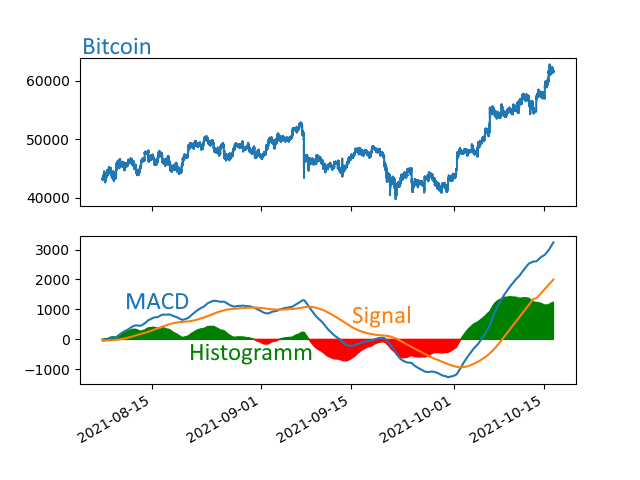
\includegraphics[width=\linewidth]{macd.png}
			\caption{Calculation of MACD}
			\label{fig:macd}
		\end{figure}
		In der Fachsprache ist ein Indikator ein Anzeichen für eine bestimmte Entwicklung oder einen eingetretenen Zustand. (\cite{OxfordLanguageIndicator}) Bei Indikatoren im Cryptotrading geht es auch um Zustände beziehungsweise die Entwicklung dieser, zum Beispiel das Erkennen eines Trends, Berechnen von möglichen Kauf- und Verkaufssignalen oder zur Risikobestimmung. Auch die Interpretation von Indikatoren kann auf viele verschiedene Arten erfolgen, oft nutzt man zum Beispiel Schwellenwerte, um die Ergebnisse von Indikatoren in bestimmte Trends oder Signale zu unterteilen.\\
		Ein weit verbreiteter Indikator ist der\glqq MACD.\grqq{}, kurz für\glqq Moving Average Convergence Divergence\grqq{} (\cite{investopediaMACD}), zu deutsch\glqq Indikator für das Zusammen- und Auseinanderlaufen des gleitenden Durchschnitts.\grqq{} (\cite{wikipediaMACDDeutsch})\\ Die Berechnung des MACD besteht ausschließlich aus einer Kombination von sogenannten \glqq EMAs\grqq{}, kurz für \glqq eponential weighted moving average\grqq{}. Dieses wird berechnet, indem man zuerst eine Zeitperiode und einen Wichtungsfaktor, meist zwei für eine quadratische Wichtung, wählt. Dividiert man den Wichtungsfaktor durch die Zeitperiode um eins erhöht, so erhält man den Glättungsfaktor für das EMA. Um die eigentliche EMA-Linie zu berechnen, wird dann aus den ältesten Werten von der vorher gewählten Zeitperiode der Mittelwert errechnet. Damit sind alle Grundvoraussetzungen erfüllt und jeder weitere Wert ergibt sich aus der EMA-Formel: der aktuelle Cryptowert minus den vorherigen EMA-Wert und das Ergebnis multipliziert mit dem bereits berechneten Glättungsfaktor. Dazu wird schließlich noch der letzte EMA-Wert addiert.\\
		Um mithilfe dieser gewichteten Rundungsfunktionen die wesentlichen Kaufsignale herauszuarbeiten, bedient man sich nun des MACD. Dafür werden zuerst der so genannte\glqq slow EMA\grqq{} und der\glqq fast EMA\grqq{} berechnet. Sie unterscheiden sich nur in ihrer Periodendauer, allerdings gibt es verschiedene populäre Konfigurationen des MACDs mit unterschiedlichen EMA-Perioden. Häufig wird für das schnelle EMA eine Zeit von zwölf Tagen und für das langsame eine von sechsundzwanzig verwendet.\\
		Die Differenz beider EMAs bildet die MACD-Line\\
		Mit einem EMA von meist neun Tagen wird aus der MACD-Line die Signal-Line berechnet. Durch die erneute Rundung scheint die Signal-Line wesentlich träger als die MACD-Line.\\
		Zu guter Letzt ergibt sich aus der Differenz von MACD-Line und Signal-Line das Histogramm.
	\subsubsection{Auswertung des MACDs}
		Wann immer MACD-Line und Histogramm einander schneiden, schneidet das Histogramm die X-Achse. Je nach dem ob es in den positiven oder den negativen Bereich schneidet, ergeben sich Kauf- und Verkaufssignal. Die simpelste Methode der Auswertung ist es, wann immer das Histogramm positiv ist, eine Position zu kaufen, und wann immer es in den negativen Bereich geht wieder zu verkaufen.
		\begin{figure}
			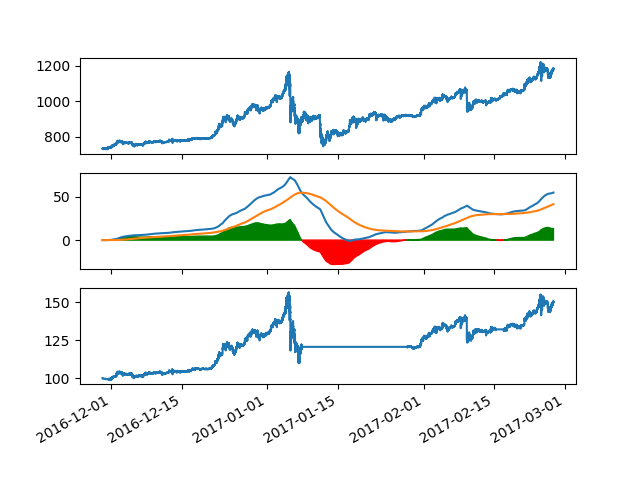
\includegraphics[width=\linewidth]{macd_resulte_btc.png}
			\caption{Gewinne bei Anwendung des MACD}
			\label{fig:macd2}
		\end{figure}
		Beim Backtesting lässt sich gut erkennen, dass der MACD im Beispiel des Bitcoin in Teilen von 2016/17 einen guten Gewinn von 50 Prozent erwirtschaftet.
	
\section{Resümee}
	Wozu einen Algorithmus mit nur einem Indikator? Ist das etwas Neues?\\
	Zwar ist die Anwendung des MACD keine besondere Sache, jedoch birgt ein solches Programm mehr Potential in sich, als man von vornherein vermuten mag. Durch seine modulare Programmierung lassen sich ohne Aufwand bestimmte Teile austauschen. Das betrifft zum einen die Indikatoren. Die Datenverarbeitung und Eingabe sowie die Indikatorfunktion sind bereits programmiert. Um einen weiteren Indikator hinzuzufügen, ist es also nur noch nötig, die Formeln in Scriptform umzusetzen. Auch die Auswertung nimmt selbst definierte Auswertungsfunktionen an, wobei die simple Deutung des MACD, die dort aktuell verwendet wird, nur ein Platzhalter ist. Es lassen sich Funktionen übergeben, die beispielsweise mehrere Indikatoren unterschiedlich und dynamisch wichten.\\
	Das größte Potential liegt jedoch in der Effizienz. Zwar ist der Algorithmus nicht außergewöhnlich schnell, aber nichts desto Trotz schnell genug, um auf einem durchschnittlichen Computer eine Millionen Werte in weit unter einer Minute zu verarbeiten. Eine Möglichkeit, einen Nutzen daraus zu ziehen, wäre, die Indikatoren während der Laufzeit auf jede Währung einzeln und permanent neu dynamisch zu bewerten. Es gibt keine allgemein beste Konfiguration von Indikatoren, allein schon wegen des Unterschiedlichen Verhaltens unterschiedlicher Cryptowährungen. Jedoch wäre es eine Möglichkeit, zu jeder Währung zu jedem Zeitpunkt eine passende Konfiguration verschiedener angepasster Indikatoren zu verwenden. Aus der stetig wachsenden Menge an vergangenen Cryptowerten lassen sich ohne Aufwand alle Werte für das Trading in der Gegenwart anpassen.\\
	Um sich nicht komplett auf die unvorhersehbare Performance der Indikatoren zu verlassen, bietet es sich trotzdem an, eine Sicherung einzubauen, die zum Beispiel bei einer gewissen negativen Abweichung von der Erwartung die Position verkauft oder gegebenenfalls manuelle Eingaben empfängt. Die Möglichkeiten gehen viel weiter und es gibt unzählige Kombinationen zu erproben. Der Algorithmus mag zwar simpel wirken, und das ist er auch, das heißt allerding nicht, dass er kein großes Potential in sich birgt.

\newpage
\nocite{*}
\printbibliography[heading=bibintoc,title=Literaturverzeichnis,notkeyword={picture}]
\printbibliography[heading=bibintoc,title=Bildverzeichnis,keyword={picture}]

\newpage
\section{Selbstständigkeitserklärung}
	Hiermit erkläre ich, dass ich die vorliegende Seminararbeit selbstständig und ohne fremde Hilfe verfasst und keine anderen Hilfsmittel als die angegebenen verwendet habe.
	Insbesondere versichere ich, dass ich alle wörtlichen und sinngemäßen Übernahmen aus anderen Werken – dazu gehören auch Internetquellen – als solche kenntlich gemacht habe.\\\\
	\_\_\_\_\_\_\_\_\_\_\_\_\_\_\_\_\_\_\_\_\_\_\_\_\_\_\_\_\_\_\_\_\_\_\_\_\\
	(Ort, Datum)\\\\
	\_\_\_\_\_\_\_\_\_\_\_\_\_\_\_\_\_\_\_\_\_\_\_\_\_\_\_\_\_\_\_\_\_\_\_\_\\
	(Unterschrift) 

\end{document}

